\documentclass[12pt,border=3mm]{standalone}
\usepackage[T1]{fontenc}
\usepackage{lmodern,amsmath,amssymb,tikz}
\usetikzlibrary{arrows.meta,positioning,calc}
\linespread{1.2}
\begin{document}
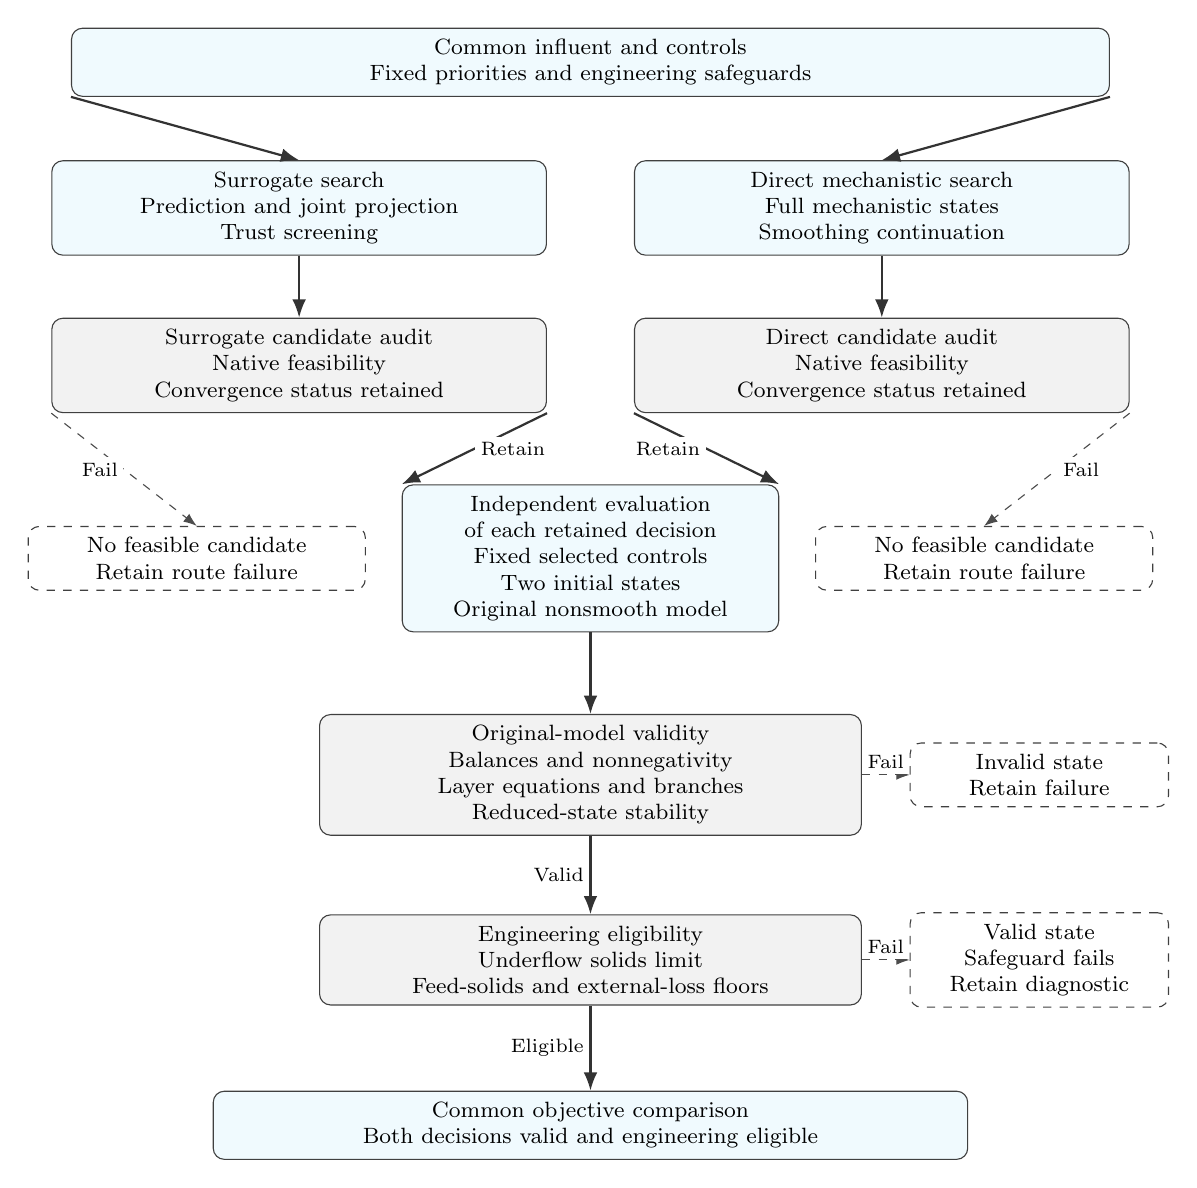
\begin{tikzpicture}[>=Latex,
block/.style={draw=black!75,rounded corners,fill=cyan!6,align=center,font=\footnotesize,inner sep=4pt},
audit/.style={block,fill=black!5},
failure/.style={block,dashed,fill=white},
flow/.style={->,thick,draw=black!80},
failflow/.style={->,dashed,draw=black!70},
lab/.style={font=\scriptsize,fill=white,inner sep=2pt}]
\node[block,text width=12.9cm] (common) at (0,0)
{Common influent and controls\\Fixed priorities and engineering safeguards};
\node[block,text width=6.0cm] (surrogate) at (-3.7,-1.85)
{Surrogate search\\Prediction and joint projection\\Trust screening};
\node[block,text width=6.0cm] (direct) at (3.7,-1.85)
{Direct mechanistic search\\Full mechanistic states\\Smoothing continuation};
\node[audit,text width=6.0cm] (snative) at (-3.7,-3.85)
{Surrogate candidate audit\\Native feasibility\\Convergence status retained};
\node[audit,text width=6.0cm] (mnative) at (3.7,-3.85)
{Direct candidate audit\\Native feasibility\\Convergence status retained};
\node[failure,text width=4.0cm] (sfail) at (-5.0,-6.3)
{No feasible candidate\\Retain route failure};
\node[failure,text width=4.0cm] (mfail) at (5.0,-6.3)
{No feasible candidate\\Retain route failure};
\node[block,text width=4.5cm] (evaluate) at (0,-6.3)
{Independent evaluation\\of each retained decision\\Fixed selected controls\\Two initial states\\Original nonsmooth model};
\node[audit,text width=6.6cm] (valid) at (0,-9.05)
{Original-model validity\\Balances and nonnegativity\\Layer equations and branches\\Reduced-state stability};
\node[failure,text width=3.0cm] (invalid) at (5.7,-9.05)
{Invalid state\\Retain failure};
\node[audit,text width=6.6cm] (engineering) at (0,-11.4)
{Engineering eligibility\\Underflow solids limit\\Feed-solids and external-loss floors};
\node[failure,text width=3.0cm] (engfail) at (5.7,-11.4)
{Valid state\\Safeguard fails\\Retain diagnostic};
\node[block,text width=9.3cm] (comparison) at (0,-13.5)
{Common objective comparison\\Both decisions valid and engineering eligible};
\draw[flow] (common.south west)--(surrogate.north);
\draw[flow] (common.south east)--(direct.north);
\draw[flow] (surrogate)--(snative);
\draw[flow] (direct)--(mnative);
\draw[flow] (snative.south east)--(evaluate.north west) node[midway,right,lab] {Retain};
\draw[flow] (mnative.south west)--(evaluate.north east) node[midway,left,lab] {Retain};
\draw[failflow] (snative.south west)--(sfail.north) node[midway,left,lab] {Fail};
\draw[failflow] (mnative.south east)--(mfail.north) node[midway,right,lab] {Fail};
\draw[flow] (evaluate)--(valid);
\draw[flow] (valid)--(engineering) node[midway,left,lab] {Valid};
\draw[failflow] (valid)--(invalid) node[midway,above,lab] {Fail};
\draw[flow] (engineering)--(comparison) node[midway,left,lab] {Eligible};
\draw[failflow] (engineering)--(engfail) node[midway,above,lab] {Fail};
\end{tikzpicture}
\end{document}
